% Define the document type and font size
\documentclass[12pt]{article}

\usepackage[spanish]{babel} % Package for the Spanish language
\usepackage[utf8]{inputenc} % Package for UTF-8 character encoding
\usepackage{geometry} % Package to configure document margins
\usepackage{graphicx} % Package to include graphics
\usepackage{listings} % Package to include source code in the document
\usepackage{xcolor} % Package to define colors
\usepackage{fancyhdr} % Package to customize headers and footers
\usepackage{amsmath} % Package for advanced mathematical symbols and environments
\usepackage{amssymb} % Package for additional mathematical symbols
\usepackage[hidelinks]{hyperref} % Package for hyperlinks in index and references (Keep this as the last package loaded)

\setlength{\parskip}{1em} % Space between paragraphs
\setlength{\parindent}{0.0in} % Indentation for paragraphs

% Definition of colors for source code
\definecolor{COLOR_COMMENTS}{HTML}{999999}
\definecolor{COLOR_KEYWORDS}{HTML}{37a5a6}
\definecolor{COLOR_IDENTIFIERS}{HTML}{ea76cb}
\definecolor{COLOR_STRINGS}{HTML}{ff7858}

% Configuration of the listings environment to display source code
\lstset{
frame=shadowbox,
aboveskip=3mm,
belowskip=3mm,
xleftmargin=10mm,
xrightmargin=10mm,
showstringspaces=false,
columns=flexible,
basicstyle={\footnotesize\ttfamily},
numbers=left,
numberstyle=\tiny\color{COLOR_COMMENTS},
keywordstyle=\color{COLOR_KEYWORDS},
stringstyle=\color{COLOR_STRINGS},
commentstyle=\color{COLOR_COMMENTS},
breaklines=true,
breakatwhitespace=true,
tabsize=4,
}

% Configuration of document margins
\geometry{
    a4paper,
    left=25mm,
    right=25mm,
    top=25mm,
    bottom=25mm
}
\graphicspath{{../img}} % Path for images

\title{El Algoritmo de PageRank de Google} % Document title
\author{María Laura Reina y Victoria Ruza} % Document author
\date{\today} % Document date

\begin{document}

    \begin{titlepage}
        \centering
        {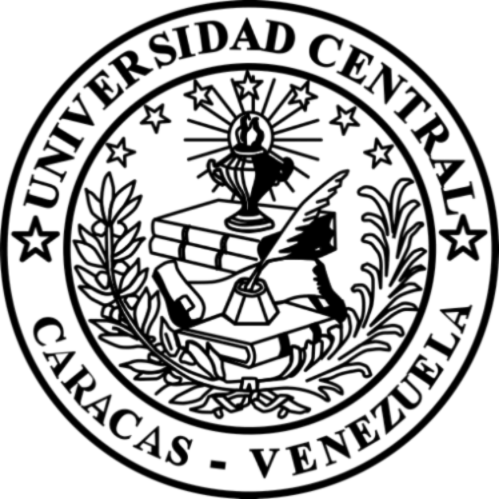
\includegraphics[width=0.2\textwidth]{logoBlack}\par}
        {\large {Universidad Central de Venezuela}\par}
        {\large {Facultad de Ciencias}\par}
        {\large {Escuela de Computación}\par}
        {\large {Cálculo Científico}\par}
        \vfill
        {\Huge {El Algoritmo de PageRank de Google}\par}
        \vfill
        {\large María Laura Reina y Victoria Ruza\par}
        \vspace{0.5cm}
        {\large \today\par}
    \end{titlepage}

    \pagenumbering{gobble}
    \tableofcontents
    \newpage
    \pagenumbering{arabic}

    \section{Objetivos}
        \subsection{Objetivo General}
            \begin{itemize}
                \item Implementar el algoritmo de PageRank para determinar la importancia relativa de los nodos en un grafo dirigido.
            \end{itemize}
        \subsection{Objetivos Específicos}
            \begin{itemize}
                \item Comprender los fundamentos matemáticos detrás del algoritmo de PageRank, la matriz de transición y el vector de rangos.
                \item Alcanzar la convergencia del algoritmo de PageRank mediante el método de las potencias y su relación con el factor de amortiguamiento.
                \item Aplicar el algoritmo de PageRank a diferentes grafos dirigidos y analizar los resultados obtenidos.
            \end{itemize}

    \newpage

    \section{Implementación computacional}
        La implementación computacional del algoritmo de PageRank se realizó en Python, utilizando la librería \texttt{NumPy} para el manejo eficiente de matrices y vectores.

        Se definió una función \texttt{pageRank} que recibe como parámetros la matriz de transición \texttt{M} correspondiente al grafo, el factor de amortiguamiento \texttt{d} y el número máximo de iteraciones \texttt{maxIter}.

        La función se encarga de identificar aquellas columnas de la matriz cuya suma es cero, es decir, aquellas páginas que no tienen enlaces salientes. Para estas columnas, se reemplaza su contenido por un vector de unos dividido por el número total de páginas, asegurando así que la matriz de transición sea estocástica.
        
        Se inicializa un vector de rangos \texttt{v} con valores iguales a $1/n$, donde $n$ es el número de páginas. Luego, se realiza un bucle de iteraciones en el que se actualiza el vector de rangos según el método de las potencias, utilizando la ecuación de PageRank:

        $$
        \mathbf{v}^{(k+1)} = d M \mathbf{v}^{(k)} + \frac{1-d}{n} \mathbf{1}
        $$

        En este bucle es incluida una re-normalización numérica del vector de rangos para mantener la suma de sus elementos igual a 1, mitigando así los errores de redondeo que puedan surgir durante las iteraciones, además de un criterio de convergencia basado en la norma del vector diferencia entre iteraciones consecutivas.
        
        Cuando la diferencia entre el vector actual y el anterior es menor a un umbral de tolerancia (En este caso $10^{-8}$), el proceso iterativo se detiene, por el contrario, si se alcanza el número máximo de iteraciones sin converger, se emite una advertencia indicando que el algoritmo no ha convergido.

    \newpage

    \section{Análisis de resultados}
        \subsection{Grafo 1}
            \begin{figure}[!ht]
                \centering
                \begin{minipage}{.5\textwidth}
                    \centering
                    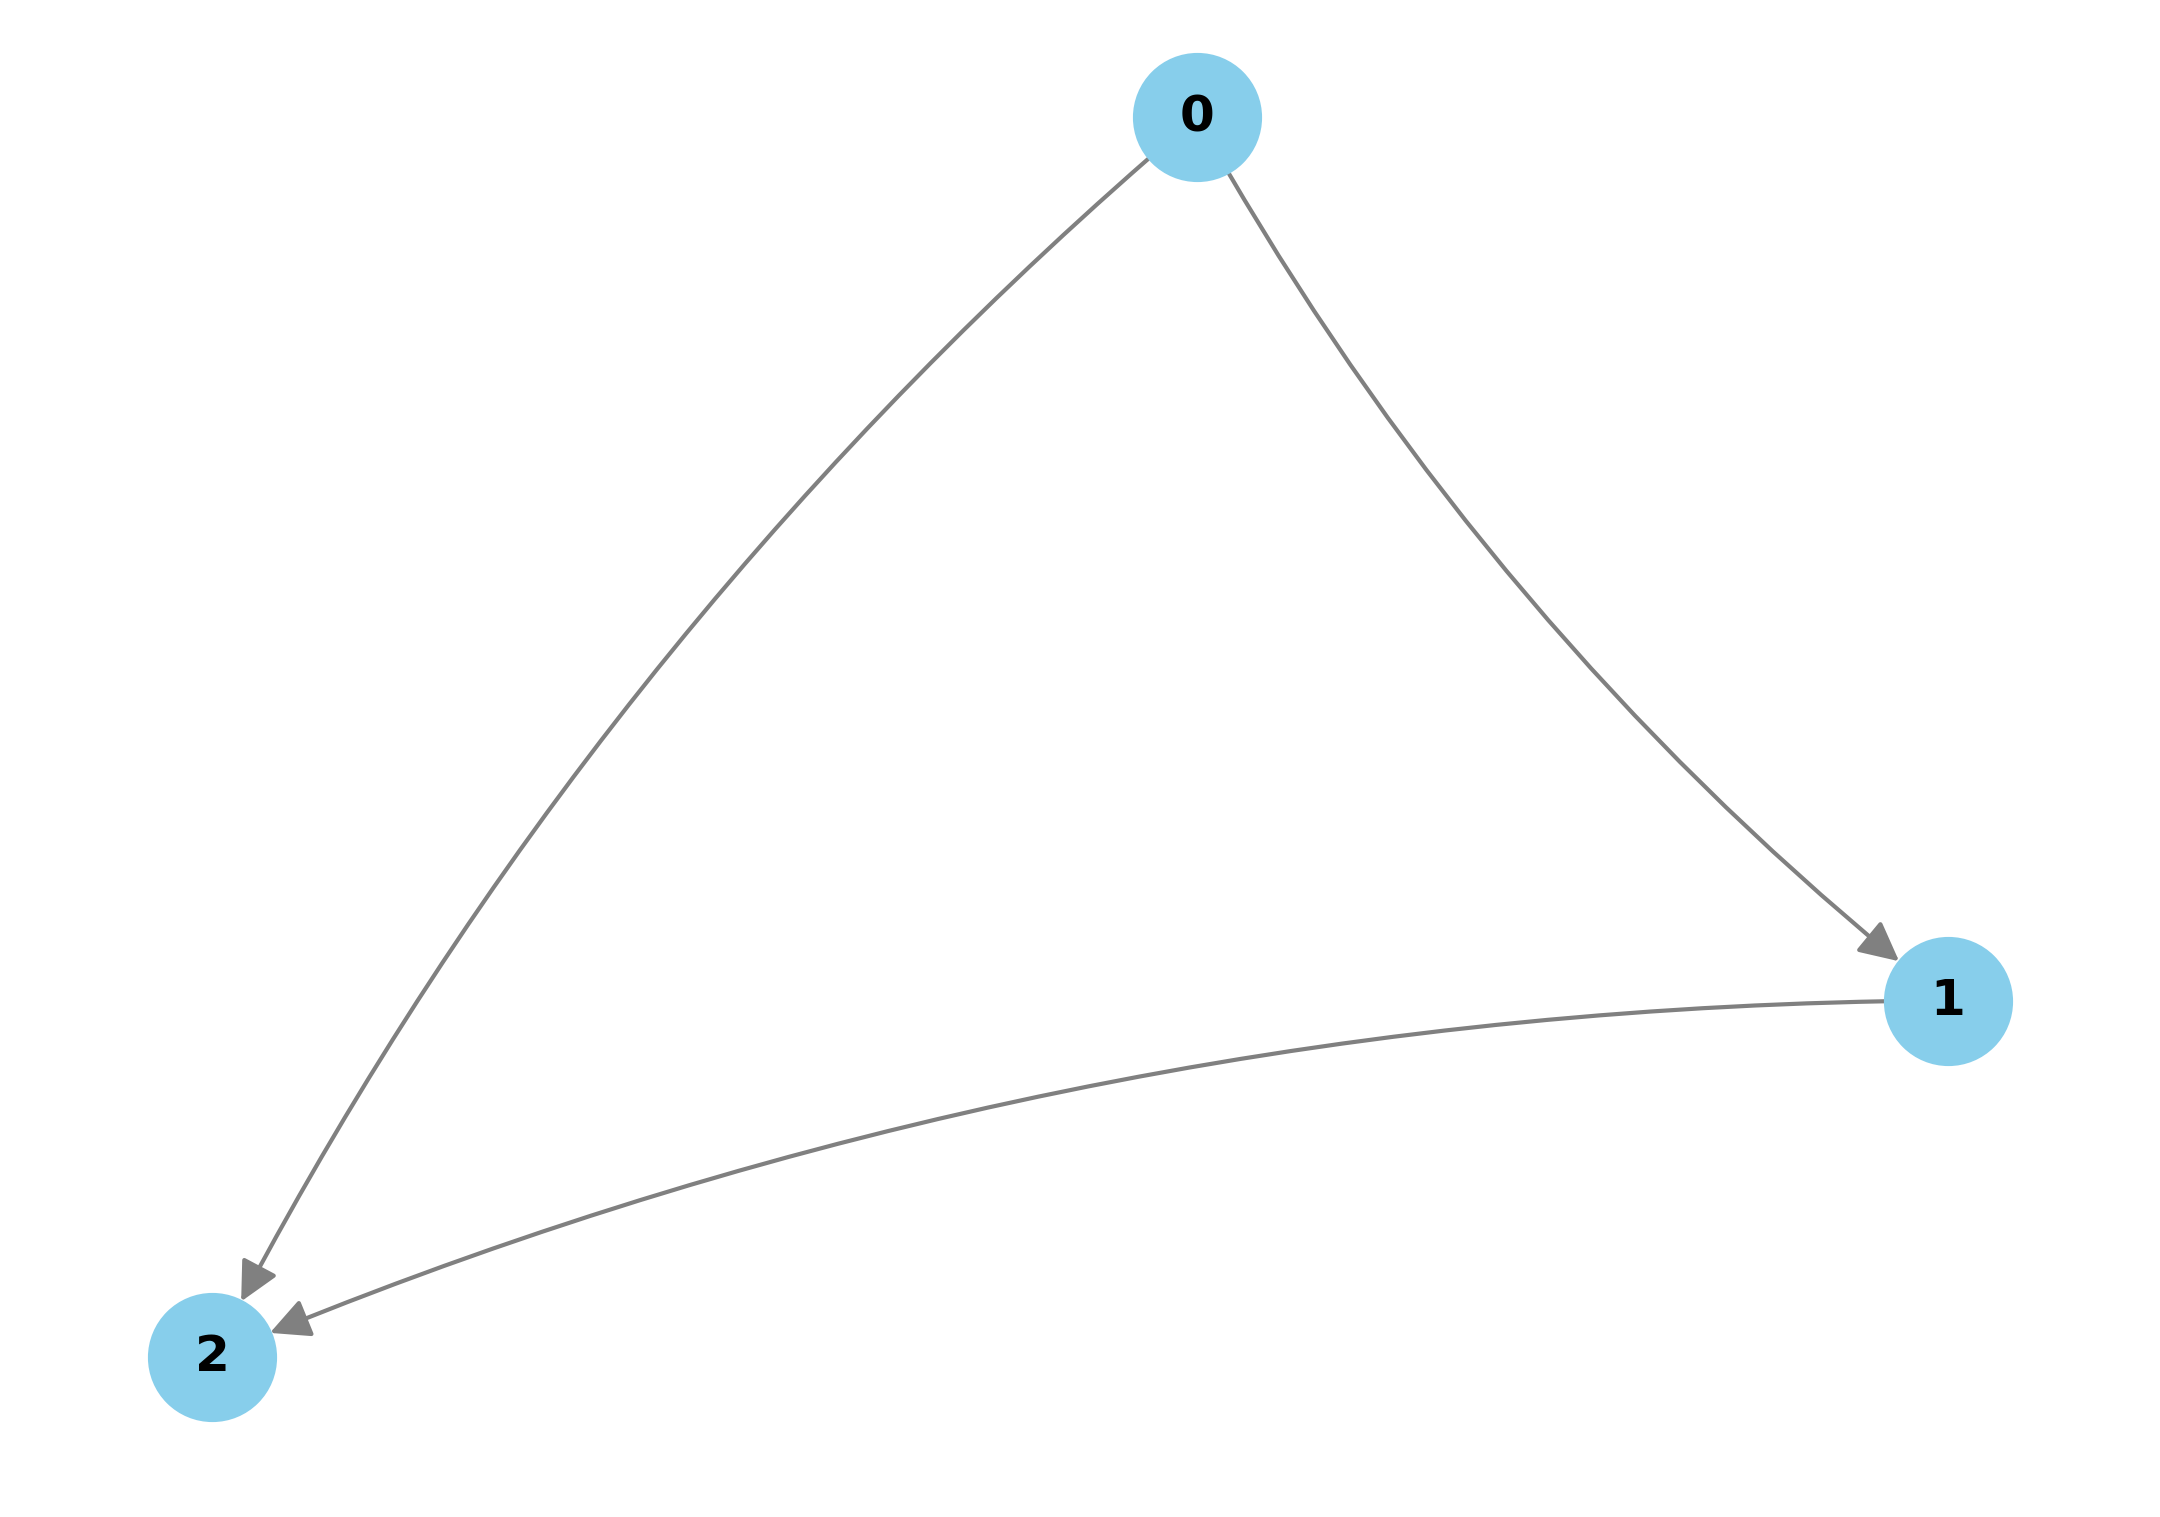
\includegraphics[width=.95\linewidth]{Casos_Pruebas/grafo_1.png}
                \end{minipage}%
                \begin{minipage}{.5\textwidth}
                    \centering
                    \begin{lstlisting}
--- Resultados para: Grafo 1 ---
-> Convergencia alcanzada en la iteracion 18 con error 4.71e-09
Vector de rangos resultante:
  Pagina 0: 0.197580 (19.76%)
  Pagina 1: 0.281551 (28.16%)
  Pagina 2: 0.520869 (52.09%)
                    \end{lstlisting}
                \end{minipage}%
            \end{figure}

            El vector de rangos resultante de aplicar el algoritmo PageRank en el grafo 1 indica que el nodo 2 ocupa la posición más alta, seguido por el nodo 1, mientras que el nodo 0 se encuentra en la última posición.

            Esto se debe a que el nodo 2 tiene un enlace entrantes desde los nodos 0 y 1, que a su vez no tienen enlaces salientes a otros nodos, acumulando así una mayor importancia en el grafo.

        \subsection{Grafo 2}
            \begin{figure}[!ht]
                \centering
                \begin{minipage}{.5\textwidth}
                    \centering
                    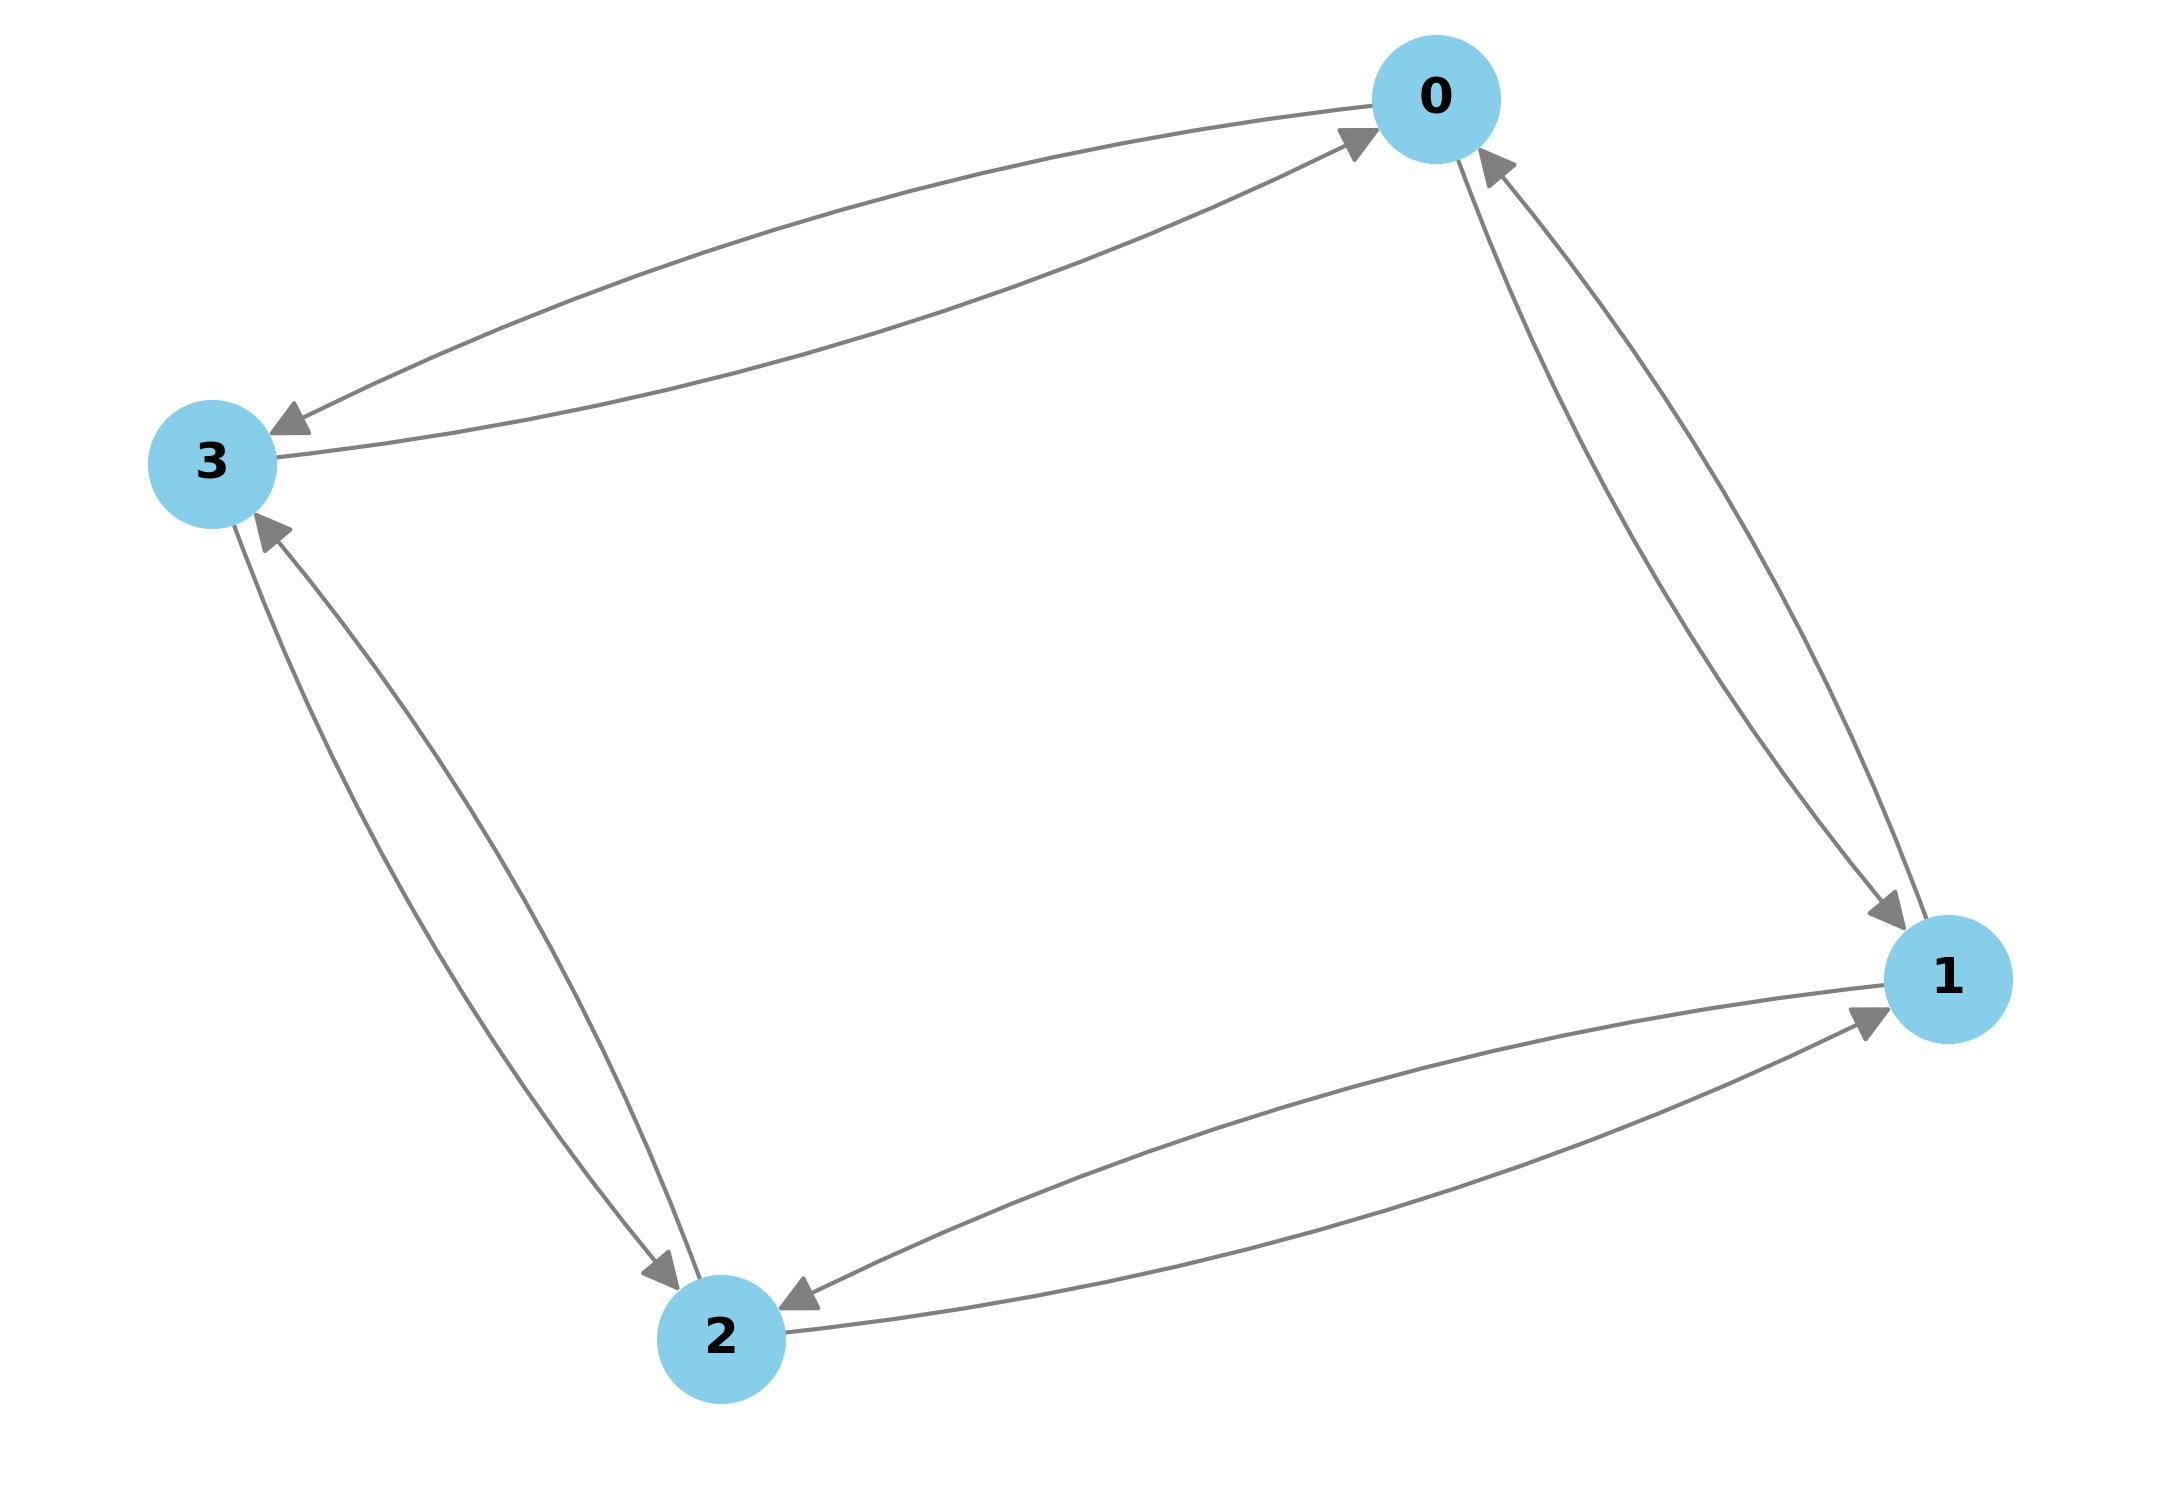
\includegraphics[width=.95\linewidth]{Casos_Pruebas/grafo_2.png}
                \end{minipage}%
                \begin{minipage}{.5\textwidth}
                    \centering
                    \begin{lstlisting}
--- Resultados para: Grafo 2 ---
-> Convergencia alcanzada en la iteracion 1 con error 0.00e+00
Vector de rangos resultante:
  Pagina 0: 0.250000 (25.00%)
  Pagina 1: 0.250000 (25.00%)
  Pagina 2: 0.250000 (25.00%)
  Pagina 3: 0.250000 (25.00%)
                    \end{lstlisting}
                \end{minipage}%
            \end{figure}

            Podemos observar un caso particular en el grafo 2, donde todos los nodos tienen la misma importancia, esto se debe a que todos comparten una misma estructura en la que cuentan con únicamente dos enlaces, uno entrante y uno saliente a nodos contiguos, distribuyendo de manera equitativa la importancia entre ellos.

        \newpage
        
        \subsection{Grafo 3}
            \begin{figure}[!ht]
                \centering
                \begin{minipage}{.5\textwidth}
                    \centering
                    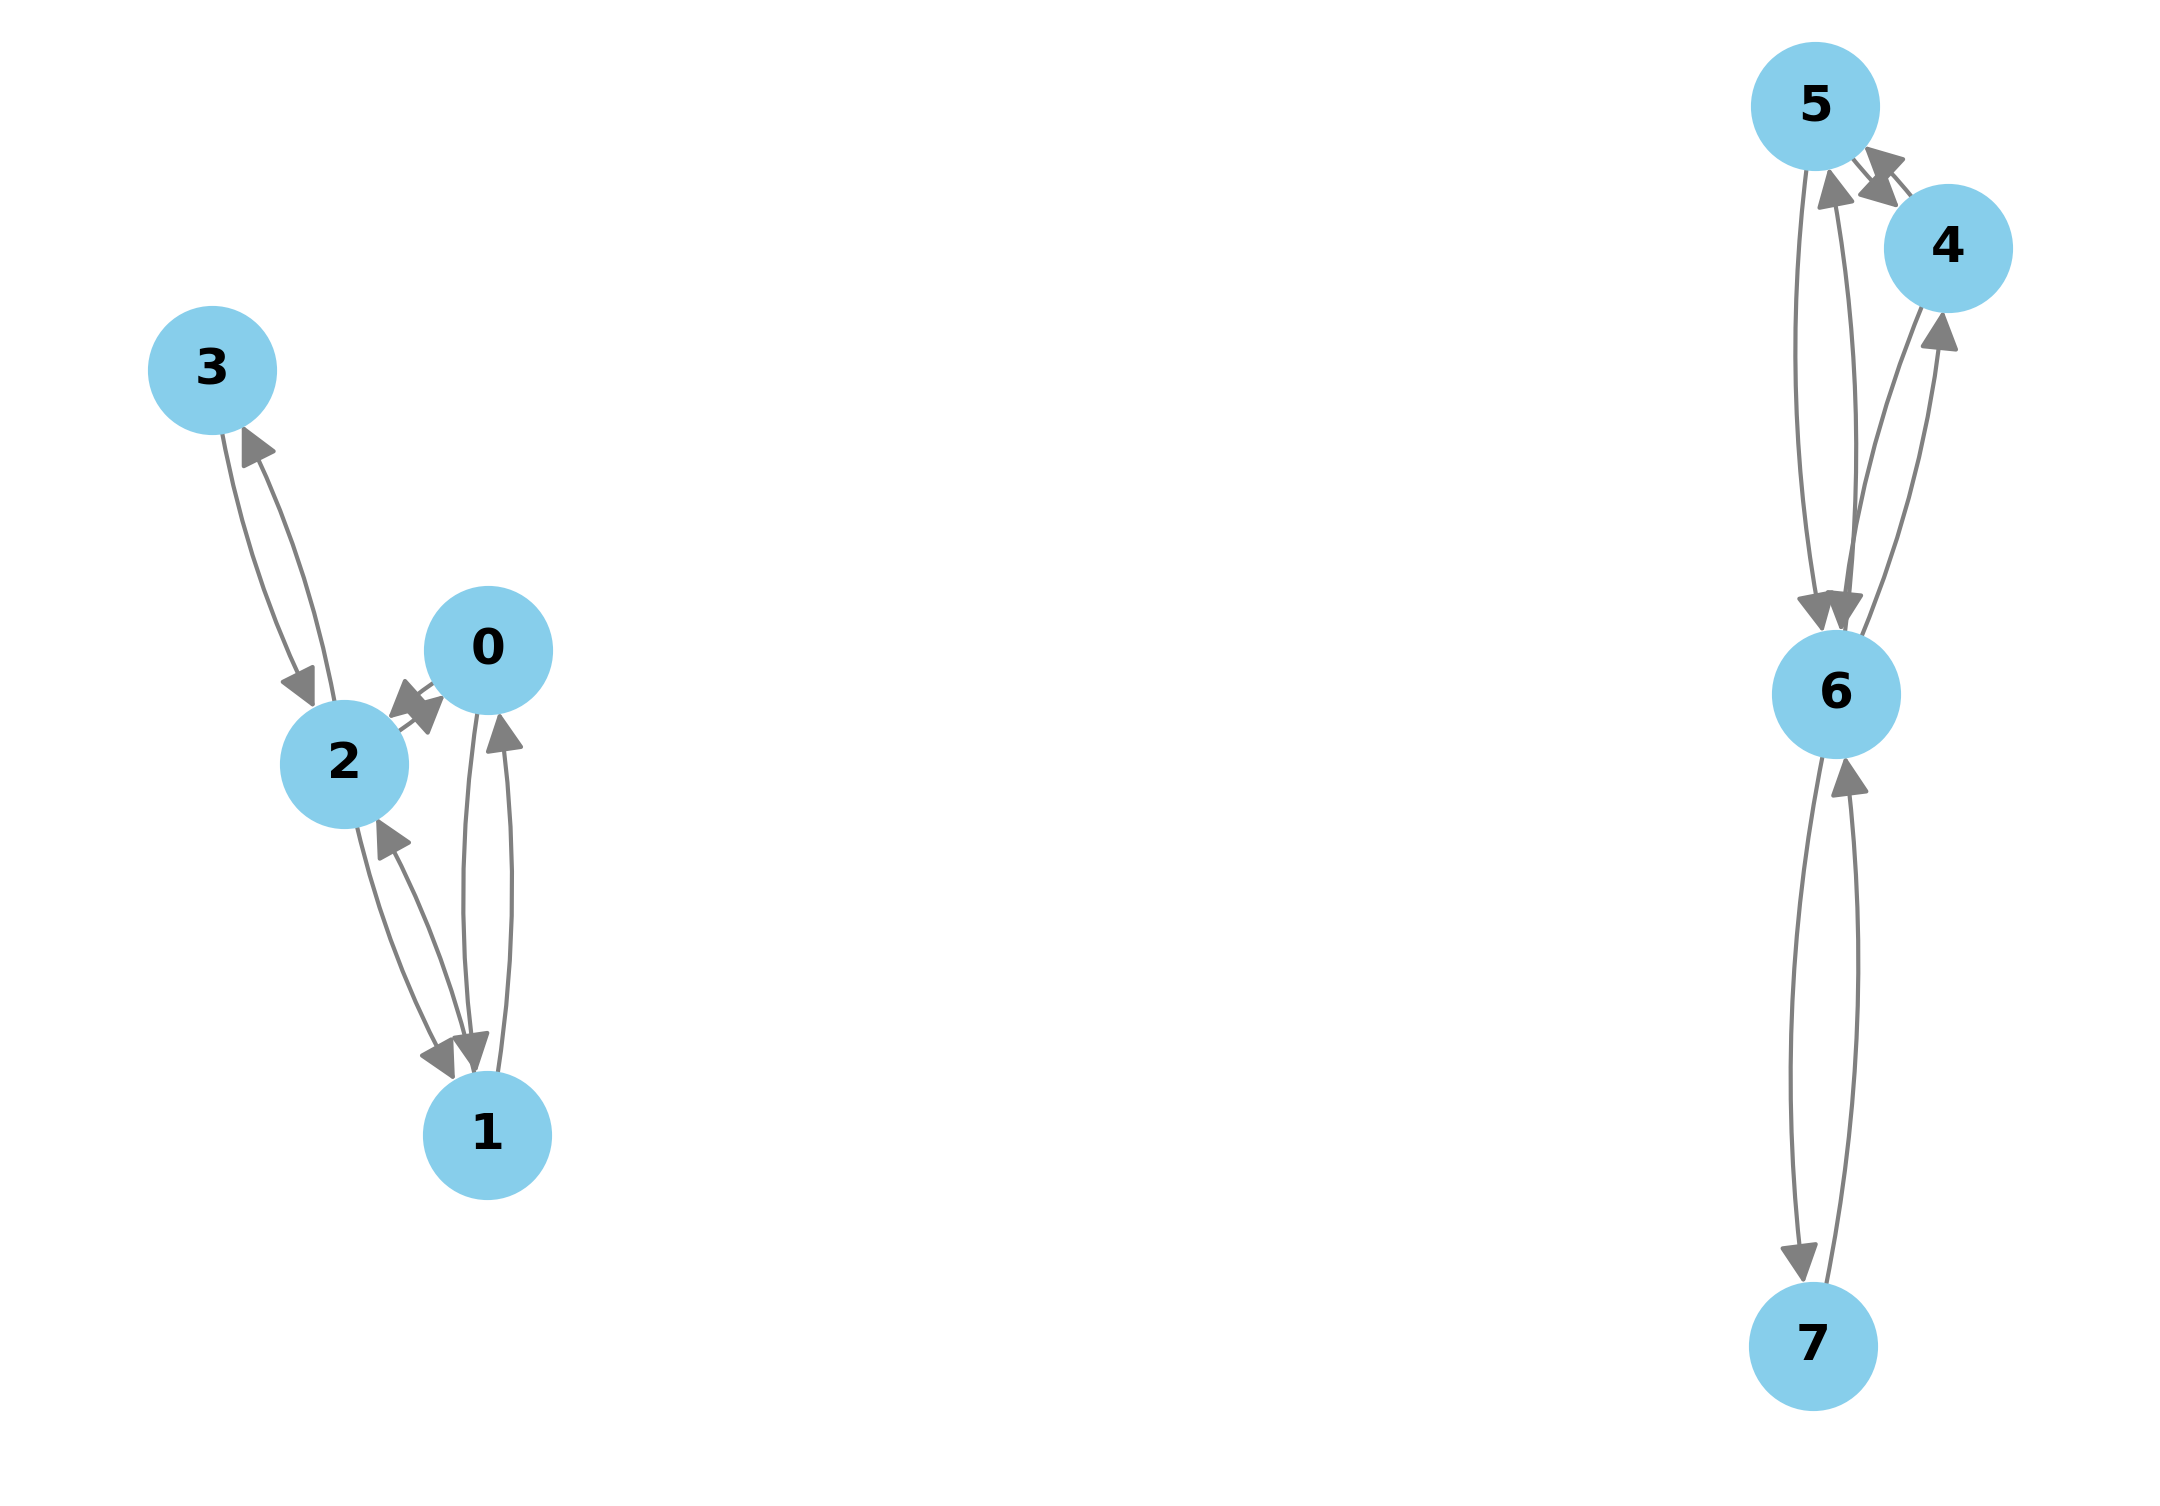
\includegraphics[width=.95\linewidth]{Casos_Pruebas/grafo_3.png}
                \end{minipage}%
                \begin{minipage}{.5\textwidth}
                    \centering
                    \begin{lstlisting}
--- Resultados para: Grafo 3 ---
-> Convergencia alcanzada en la iteracion 38 con error 9.47e-09
Vector de rangos resultante:
  Pagina 0: 0.122964 (12.30%)
  Pagina 1: 0.122964 (12.30%)
  Pagina 2: 0.183368 (18.34%)
  Pagina 3: 0.070704 (7.07%)
  Pagina 4: 0.122964 (12.30%)
  Pagina 5: 0.122964 (12.30%)
  Pagina 6: 0.183368 (18.34%)
  Pagina 7: 0.070704 (7.07%)
                    \end{lstlisting}
                \end{minipage}%
            \end{figure}

            Se puede observar que en el grafo 3, dos grupos de nodos completamente desconectados, cada uno con 4 nodos, el primero con nodos 0, 1, 2 y 3, y el segundo con nodos 4, 5, 6 y 7.

            Lo curioso en este caso es que observando los grupos individualmente, se puede notar que se comportan de manera idéntica, en la cual poseen un nodo con importancia 18.34\% (nodos 2 y 6), dos nodos con importancia 12.30\% (nodos 0, 1, 4 y 5), y finalmente un nodo con importancia 7.07 (nodos 3 y 7).

            Esto es debido a que ambos grupos de nodos poseen la misma estructura, en la cual el nodo con mayor importancia es aquel en el centro de la estructura, que posee tres enlaces entrantes y reciben importancia de todos los demás en la red, seguido de los nodos intermedios que poseen dos enlaces entrantes y salientes, recibiendo importancia del nodo central y su otro nodo adyacente y finalmente los nodos de borde que reciben importancia únicamente del nodo central.

        \subsection{Grafo 4}
            \begin{figure}[!ht]
                \centering
                \begin{minipage}{.5\textwidth}
                    \centering
                    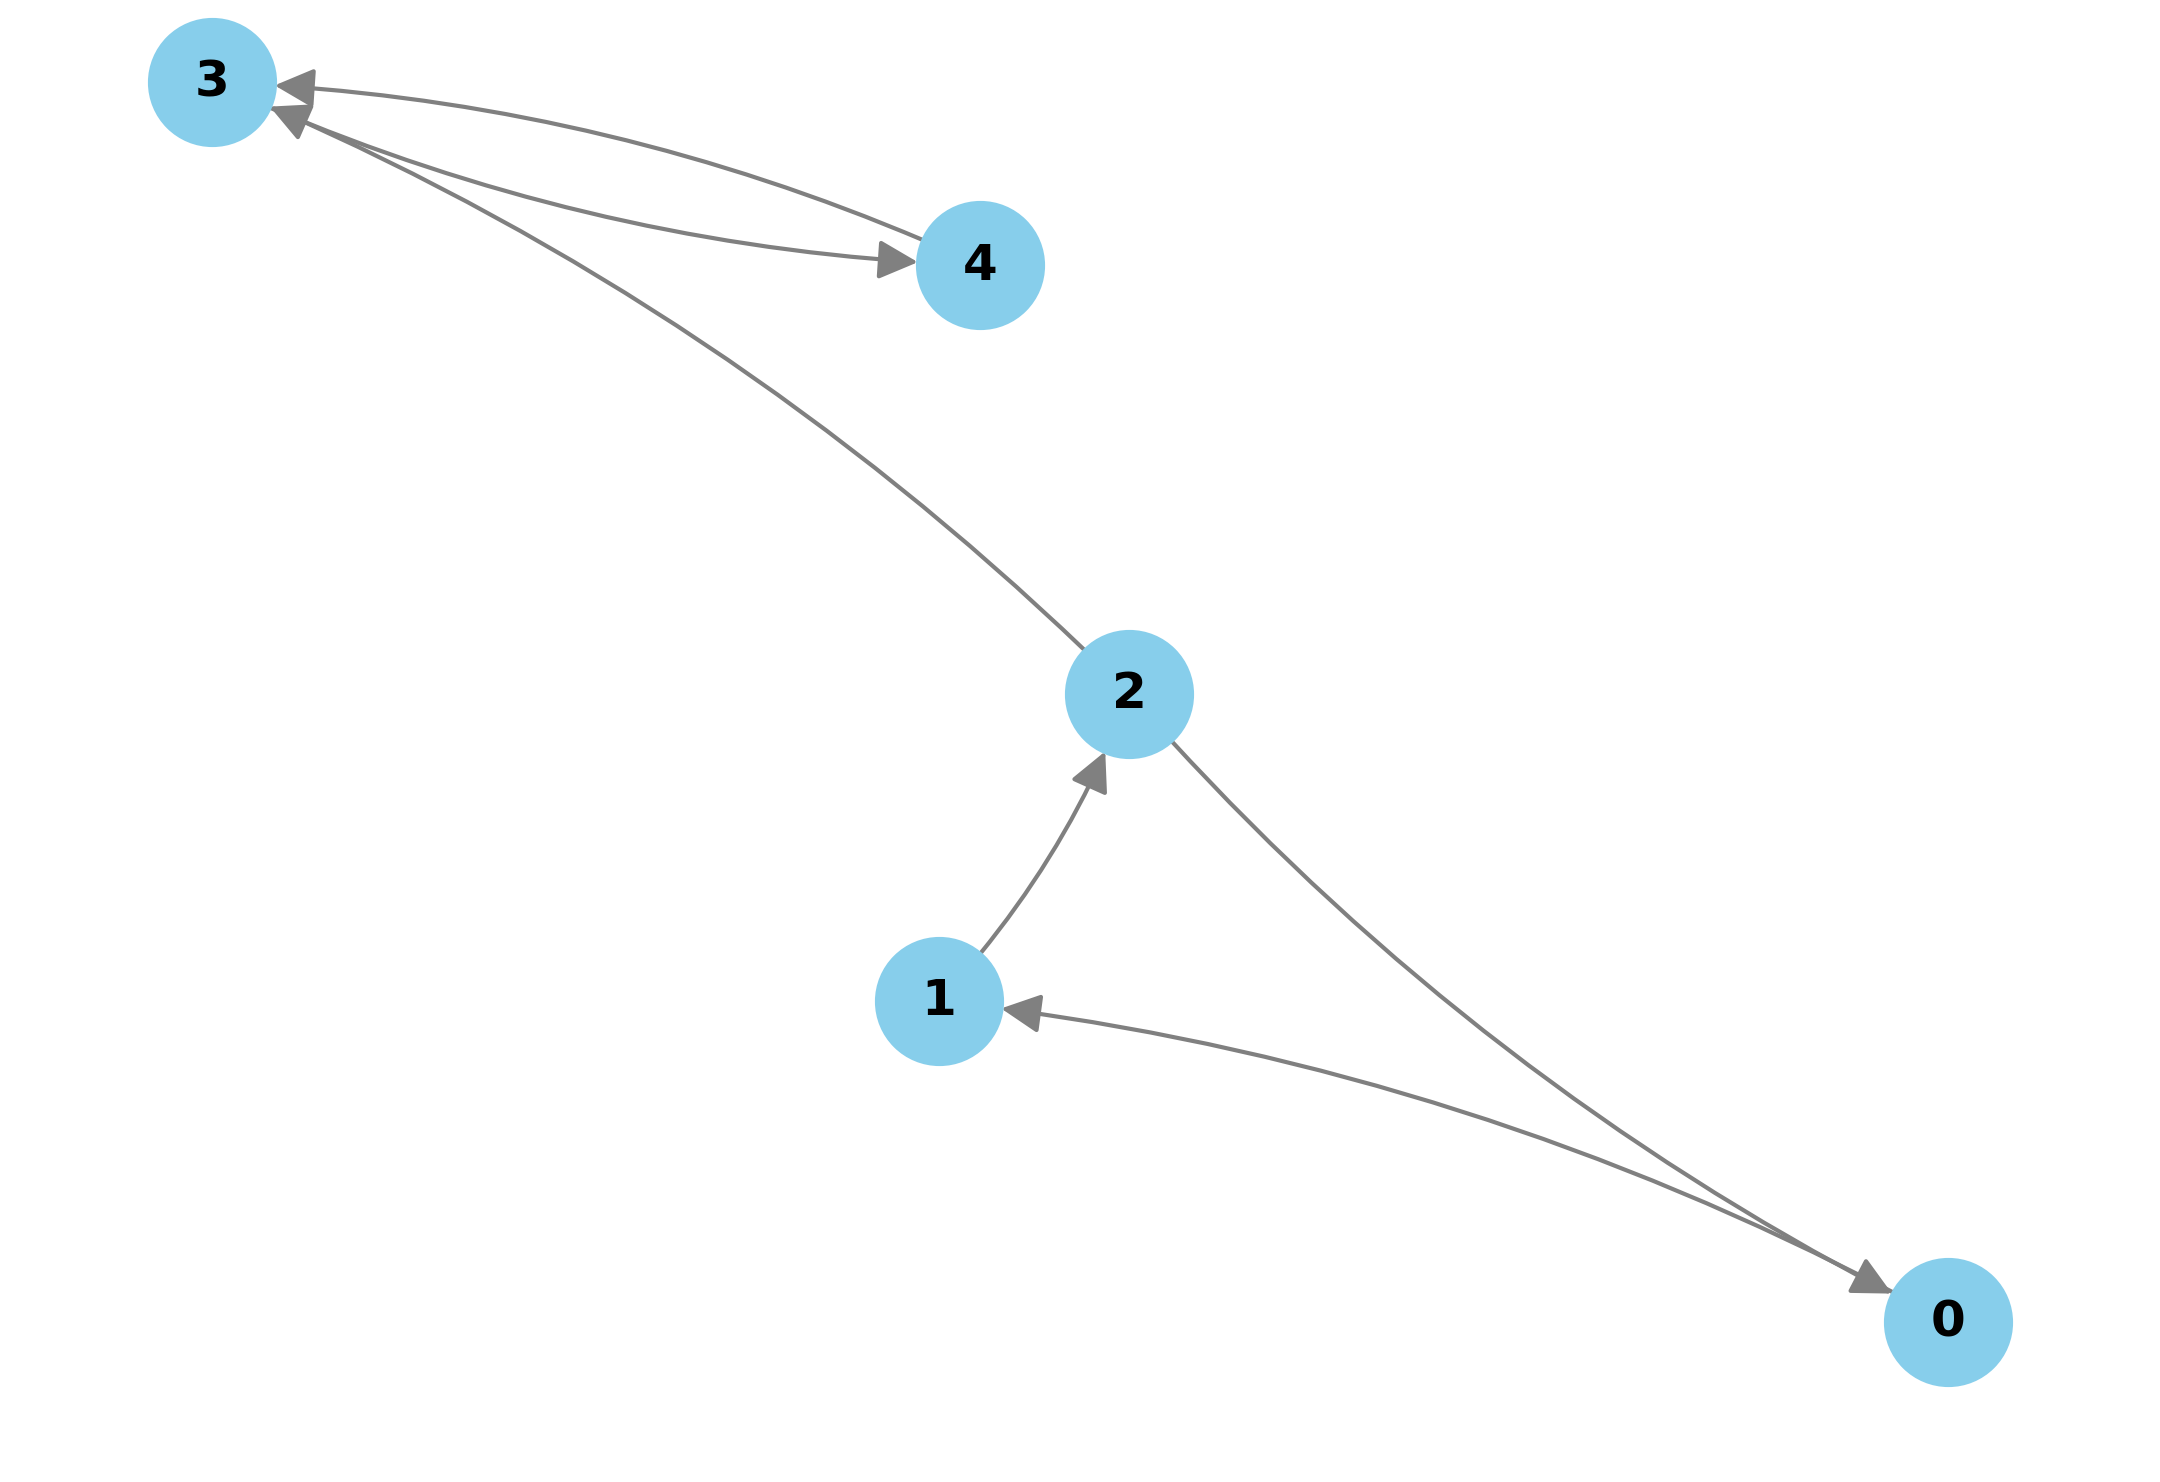
\includegraphics[width=.95\linewidth]{Casos_Pruebas/grafo_4.png}
                \end{minipage}%
                \begin{minipage}{.5\textwidth}
                    \centering
                    \begin{lstlisting}
--- Resultados para: Grafo 4 ---
-> Convergencia alcanzada en la iteracion 101 con error 9.91e-09
Vector de rangos resultante:
  Pagina 0: 0.077334 (7.73%)
  Pagina 1: 0.095734 (9.57%)
  Pagina 2: 0.111374 (11.14%)
  Pagina 3: 0.370572 (37.06%)
  Pagina 4: 0.344986 (34.50%)
                    \end{lstlisting}
                \end{minipage}%
            \end{figure}

            En el vector de rangos resultante de aplicar el algoritmo PageRank en el grafo 4, se puede observar que el nodo 3 ocupa la posición más alta, seguido por el nodo 4, estos dos nodos poseen una importancia significativamente mayor a los demás.

            Esto es debido a que si se observa el grafo correspondiente, una vez que el usuario se encuentre en el nodo 2 (Suponiendo que no salte a un nodo aleatorio debido al factor de amortiguamiento), este tiene un 50\% de probabilidad de ir al nodo 0 en el cual eventualmente terminará de vuelta en el nodo 2, y un 50\% de probabilidad de ir al nodo 3, en el cual se produce un efecto de sumidero ya que este y el nodo 4 sólo tienen enlaces salientes de uno al otro.

        \subsection{Grafo 5}
            \begin{figure}[!ht]
                \centering
                \begin{minipage}{.5\textwidth}
                    \centering
                    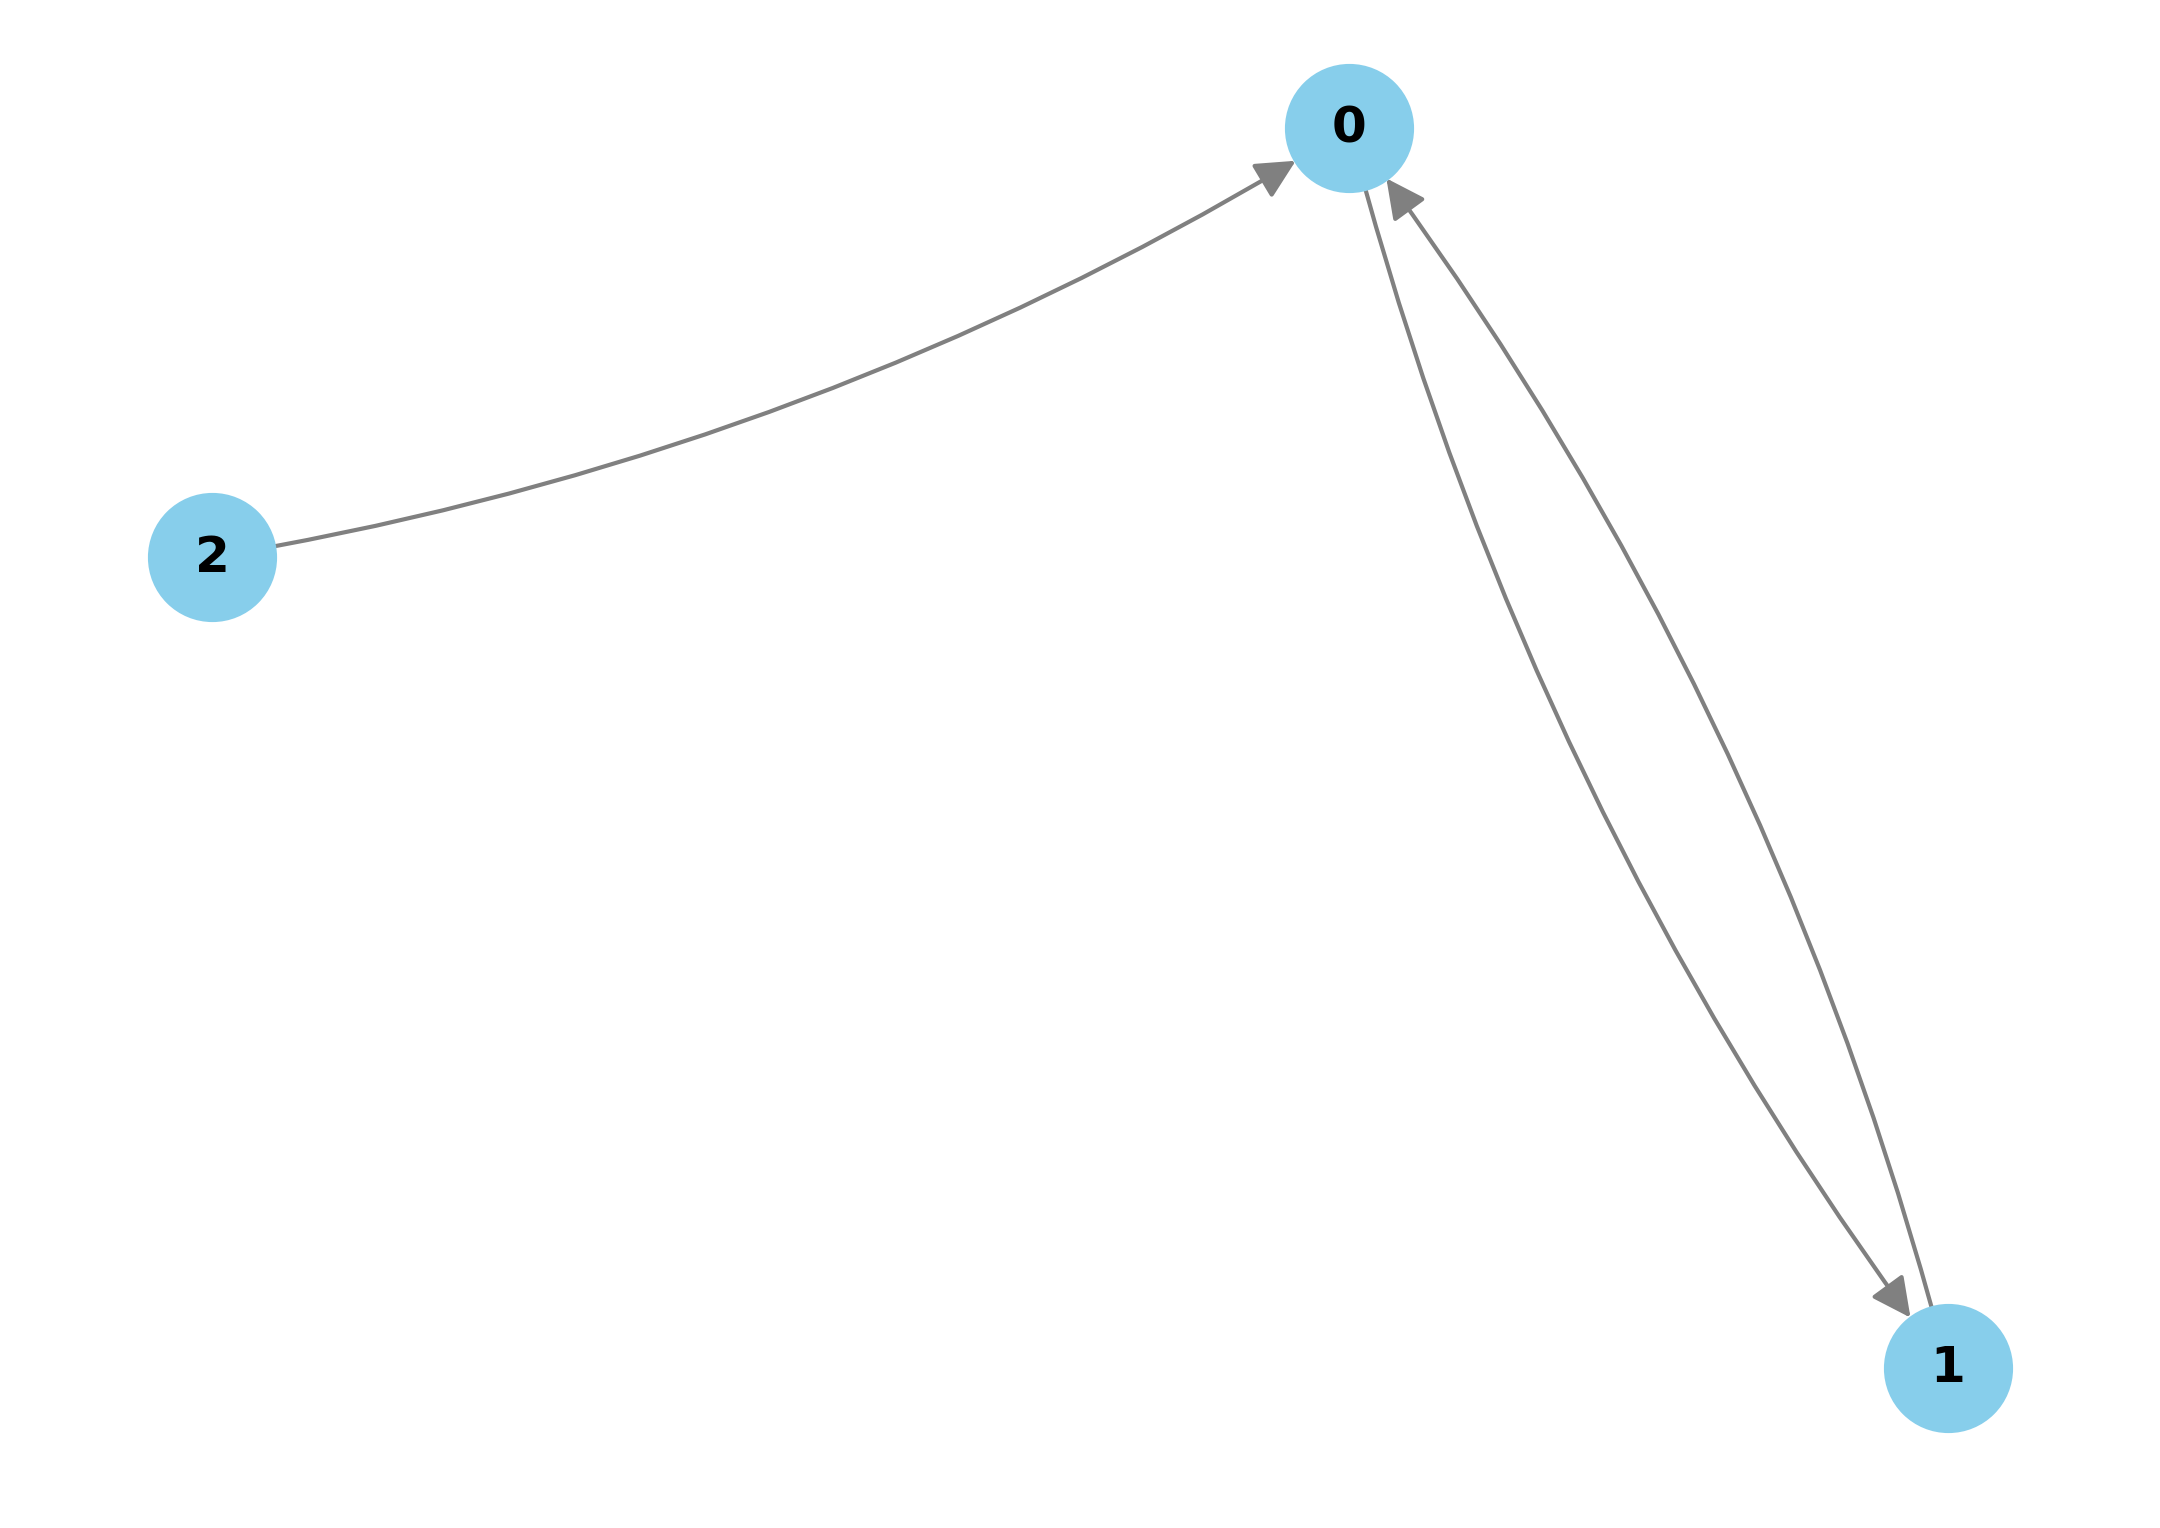
\includegraphics[width=.95\linewidth]{Casos_Pruebas/grafo_5.png}
                \end{minipage}%
                \begin{minipage}{.5\textwidth}
                    \centering
                    \begin{lstlisting}
--- Resultados para: Grafo 5 ---
-> Convergencia alcanzada en la iteracion 111 con error 9.76e-09
Vector de rangos resultante:
  Pagina 0: 0.486486 (48.65%)
  Pagina 1: 0.463514 (46.35%)
  Pagina 2: 0.050000 (5.00%)
                    \end{lstlisting}
                \end{minipage}%
            \end{figure}

            En el vector de rangos resultante de aplicar el algoritmo PageRank en el grafo 5, se puede observar que el nodo 0 ocupa la posición más alta, seguido por el nodo 1, mientras que el nodo 2 tiene la menor importancia.

            En este grafo se produce un efecto similar al ocurrido con los nodos 3 y 4 del grafo 4, en el cual los nodos 0 y 1 sólo tienen enlaces salientes de uno al otro, mientras que el nodo 2 únicamente cuenta con un enlace saliente al nodo 0 y ningún enlace entrante, por lo cual este termina acumulando importancia únicamente al ser elegido aleatoriamente por el factor de amortiguamiento, mientras que los nodos 0 y 1 acumulan importancia entre ellos y en el caso del nodo 0 también gracias al enlace proveniente del nodo 2.

        \newpage

        \subsection{Grafo Propuesto}
            \begin{figure}[!ht]
                \centering
                \begin{minipage}{.5\textwidth}
                    \centering
                    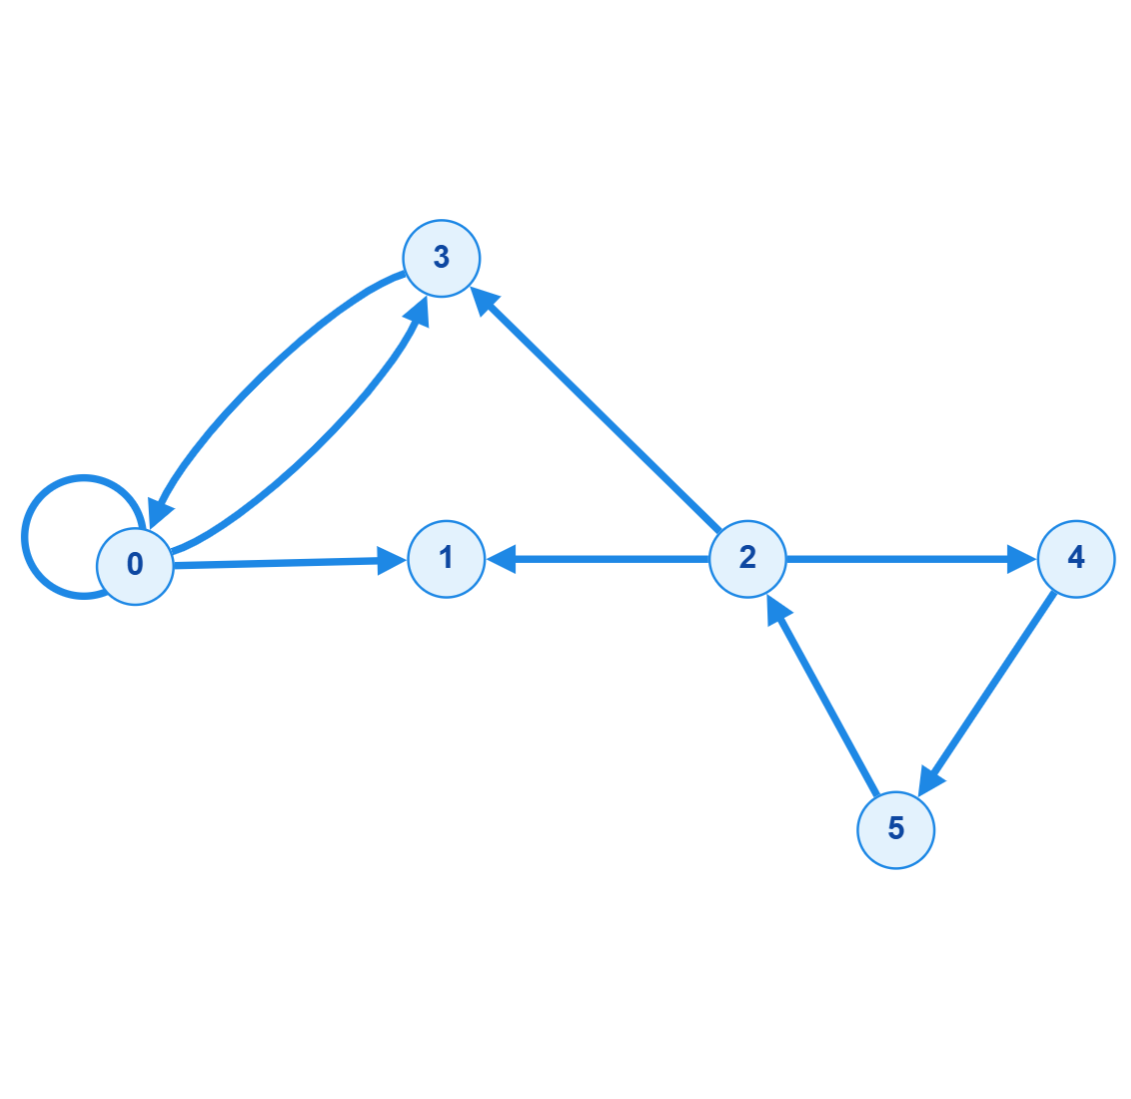
\includegraphics[width=.95\linewidth]{Casos_Pruebas/grafo_propuesto.png}
                \end{minipage}%
                \begin{minipage}{.5\textwidth}
                    \centering
                    \begin{lstlisting}
--- Resultados para: Grafo Propuesto ---
-> Convergencia alcanzada en la iteracion 34 con error 9.57e-09
Vector de rangos resultante:
  Pagina 0: 0.272586 (27.26%)
  Pagina 1: 0.171785 (17.18%)
  Pagina 2: 0.159586 (15.96%)
  Pagina 3: 0.171785 (17.18%)
  Pagina 4: 0.094552 (9.46%)
  Pagina 5: 0.129706 (12.97%)
                    \end{lstlisting}
                \end{minipage}%
            \end{figure}
                
            El grafo propuesto está conformado por 6 nodos, de los cuales el nodo 0 contiene un enlace hacia si mismo, y el nodo 1 no tiene enlaces salientes.
         
            El vector de rangos resultante de aplicar el algoritmo PageRank en el grafo propuesto indica que el nodo 0 ocupa la posición más alta, seguido por los nodos 1 y 3, mientras que el nodo 4 se encuentra en la última posición.

            El nodo 0 posee la mayor importancia a pesar de poseer un único enlace entrante a partir de otro nodo, uno pensaría que el presentar un enlace hacia si mismo le permitiría acumular importancia en el grafo, este hecho por si sólo no sería suficiente para justificar su posición, se debe además al hecho de que si el usuario se encuentra en cualquiera de los nodos 2, 3, 4 o 5, (En caso de que este no salte a un nodo aleatorio debido al factor de amortiguamiento), el usuario eventualmente terminará en el nodo 0, acumulando importancia proveniente de todos estos nodos.
            
            Bajo este mismo razonamiento, excluyendo la acumulación de importancia atribuida al bucle, es el por qué los nodos 1 y 3 poseen la segunda mayor importancia. 
            
            Por otro lado, el nodo 4 tiene la menor importancia debido a que su único enlace entrante es apartir del nodo 2 quien a su vez reparte su importancia entre el mencionado nodo 4 y el nodo 3.

        El algoritmo PageRank no decide la importancia de un nodo únicamente por la cantidad de enlaces entrantes que posee, sino que también toma en cuenta la importancia de los nodos que lo enlazan, y cómo estos a su vez distribuyen su importancia entre los demás nodos del grafo.

        Un nodo enlazado por pocos nodos de gran importancia, que a su vez no distribuyen su importancia entre muchos otros nodos, tendrá una mayor importancia que un nodo enlazado por muchos nodos de poca importancia o que distribuyen su importancia entre muchos otros nodos.

    \newpage
    \section{Referencias}
    \begin{itemize}
        \item Derivando. (2019, 1 marzo). PAGE RANK | El algoritmo matemático que hizo a GOOGLE dominar el mundo [Vídeo]. YouTube.\newline \url{https://www.youtube.com/watch?v=b3fwA3EWCd8}.
        \item Alberca, A. S. (2022, 12 mayo). La librería Numpy | Aprende con Alf. Aprende Con Alf.\newline \url{https://aprendeconalf.es/docencia/python/manual/numpy/}.
        \item Spanning Tree. (2020, June 17). How Google’s PageRank algorithm works [Video]. YouTube. \newline \url{ https://www.youtube.com/watch?v=meonLcN7LD4}.
        \item Libretexts. (2022, 2 noviembre). 5.6: Matrices estocásticas. LibreTexts Español.\newline \url{https://espanol.libretexts.org/Bookshelves/Matematicas/Algebra_lineal/%C3%81lgebra_Lineal_Interactiva_(Margalit_y_Rabinoff)/05%3A_Valores_propios_y_vectores_propios/5.05%3A_Matrices_Estoc%C3%A1sticas}.
    \end{itemize}
\end{document}
